\documentclass[../main.tex]{subfiles}
\begin{document}
    
    
    \chapter{Consumption}
    
    \section{Permanent income hypothesis (PIH)}
    
        Individual lives for $T$ periods, lifetime utility is given by
        \begin{align}
            U = \sum_{t=0}^T \frac{u(C_t)}{(1+\rho)^t}, \quad u'(\cdot) > 0, \quad u'(\cdot) < 0,
        \end{align}
        
        subject to the constraint
        \begin{align}
            \sum_{t=0}^T \frac{C_0}{\prod_{s=1}^{t} (1+r_s)}
            \le A_0 + \sum_{t=1}^T \frac{Y_t}{\prod_{s=0}^{t} (1+r_s)}, \label{eqn:constant-budget}
        \end{align}
        where $A_0$ and $\rho$ are initial wealth and time discount rate, and $C_t, Y_t,$ and $r_t$ are consumption, income, and interest rate at time $t$. Form the Lagrangian
        \begin{align}
            \L\left(\{C_t\}_{t=0}^{T}, \lambda\right)
            &= \sum_{t=0}^T
            \frac{u(C_t)}{(1+\rho)^t} + \lambda  \left(A_0 +\sum_{t=0}^T \frac{Y_t - C_t}{\prod_{s=0}^{t} (1+r_s)} \right),
        \end{align}
        
        Then with FOC with respect to consumption $C_t$ in any period $t$, we have the Euler equation
        \begin{align}
            \frac{\partial \L}{\partial C_t}
            &= \frac{u'(C_t^*)}{(1+\rho)^t} - \frac{\lambda}{\prod_{s=0}^t (1+r_s)}
            % &=
            % \frac{u'(C_t^*)}{(1+\rho)^t} - \frac{\lambda}{(1+r)^t}
            % = 0
            \\
            \implies u'(C_t^*) &= \lambda \frac{(1+\rho)^t}{\prod_{s=0}^t (1+r_s)}
            % \\
            \implies
            \frac{u'(C_t)}{u'(C_{t+1})} = \frac{1+r_{t+1}}{1+\rho}.
        \end{align}
        
        Assume $r = \rho$ for all periods, then we have that        \begin{align}
            u'(C_t)
            = \frac{1+r_{t+1}}{1+\rho} u'(C_{t+1})
            = u'(C_{t+1})
            \implies
            C_t^* = C_{t+1}^* = \bar C.
        \end{align}
        
        % Since $\lambda$ is constant across time, optimal consumption is also constant across time $t = 1, ..., T$. Then we have
        % \begin{align}
        %     C_t^* &= {u'}^{-1}(\lambda) = \bar{C}.
        % \end{align}
        
        From the budget constraint \eqref{eqn:constant-budget} (and assuming no free disposal), we have that
        \begin{align}
            \sum_{t=1}^T C_t^*
            = \sum_{t=1}^T \bar{C}
            = T \bar{C}
            &= A_0 + \sum_{t=1}^T Y_t
            \\
            \implies
            C_t^*
            =\bar{C}
            &= \frac{1}{T} \left( A_0 + \sum_{s=1}^T Y_s \right)
            = \frac{1}{T}\sum_{s=1}^T Y_s +  \frac{A_0}{T}.
        \end{align}
        
        This implies optimal consumption is not determined by income in any period $t$ but only by the total (or average) income across time. This is the \textbf{permanent-income hypothesis.} Individual savings is then
        \begin{align}
            S_t 
            = Y_t - C_t
            &= Y_t - \frac{1}{T} \left( A_0 + \sum_{s=1}^T Y_s \right)
            \\
            &= \left(Y_t -  \frac{1}{T}\sum_{s=1}^T Y_s \right) - \frac{A_0}{T}.
        \end{align}
    
    \section{Income and consumption fluctuations}
        
        Income $Y_{it}$ for individual $i$ at time $t$ can be represented as
        \begin{align}
            Y_{it} = Y_{i}^P + Y_{it}^T
            \quad s.t. \quad
            \sum_{t=1}^T Y_{it}^T = 0,\quad
            \cov{Y_{it}^T, Y_{i}^P} = 0.
            \label{eqn:income-fluctuation}
        \end{align}
        where $Y_{i}^P$ is the average across time or \textbf{permanent income}, and $Y_{it}^T = Y_{it} - Y_{i}^P$ is the \textbf{transitory income}. Assume exogenous, unexpected fluctuations in consumption. Then individual $i$ maximizes lifetime utility
        \begin{align}
            U_i &= \sum_{t=1}^T u\left(C_{it} - e_{it}\right)
             \quad s.t. \quad
            \sum_{t=1}^T \left(C_{it} - e_{it}\right) \le A_0 + \sum_{t=1}^T Y_t,
            \label{eqn:utility-fluctuation}
        \end{align}
        
        where $e_{it}$ is the \textbf{transitory consumption} (sort of like a ``consumption shock") with $\sum_{t=1}^T e_{it} = 0$. Then forming the Lagrangian, we have that
        \begin{align}
            \L
            &=
            \sum_{t=1}^T u\left(C_{it} - e_{it}\right)
            + \lambda \left[A_0 + \sum_{t=1}^T Y_t - \sum_{t=1}^T \left(C_{it} - e_{it}\right)\right]
            \\
            \frac{\partial \L}{\partial C_{it}}
            &= u'\left(C_{it}^* - e_{it}\right) - \lambda = 0
            \implies u'\left(C_{it}^* - e_{it}\right) = \lambda,
        \end{align}
        
        which implies $C_{it}^* - e_{it} = \bar{C_e}$ is constant across time also. Then with the budget constraint in \eqref{eqn:utility-fluctuation}, we have that
        
        \begin{align}
            \sum_{t=1}^T \left(C_{it} - e_{it}\right)
            &= A_0 + \sum_{t=1}^T Y_{it}
            \\ \implies
            \sum_{t=1}^T C_e
            &= A_0 + \sum_{t=1}^T (Y_{i}^P + Y_{it}^T)
            \\
            &= A_0 + \sum_{t=1}^T Y_{i}^P + \sum_{t=1}^T Y_{it}^T
            \\ \implies
            \sum_{t=1}^T \bar{C_e}
            = T \bar{C_e}
            &= A_0 + T \cdot Y_{i}^P.
        \end{align}
        
        Assuming $A_0 = 0$, we have that
        \begin{align}
            T \bar{C_e} &= T \cdot Y_{i}^P
            \\
            \implies 
            \bar{C_e} &= Y_{i}^P
            \\
            \implies
            C_{it} - e_{it} &= Y_{i}^P, \quad t = 1, ..., T
        \end{align}    
        
        Rearranging, we have the consumption function
        \begin{align}
            C_{it} &= Y_{i}^P + e_{it}, \quad t = 1, ..., T.
            \label{consumption-fluctuation}
        \end{align}
        
        
    \section{Cross-sectional regression}
    
        Running an cross-section OLS regression on $C_{it}$ with $Y_{it}$, we have
        \begin{align}
            C_{it} &= a + b Y_{it} + u_{it}
           \label{eqn:consumption-regression}
        \end{align}
        
        where with permanent income \eqref{eqn:income-fluctuation} and consumption \eqref{consumption-fluctuation}, we have
        \begin{align}
            \cov{x, y} &= \frac{1}{N}\sum_{i=1}^N(x_i - \bar{x})(y_i - \bar{y}) \\
            \var{y} &= \frac{1}{N}\sum_{i=1}^N(y_i - \bar{y})^2
        \end{align}
        \begin{align}
            \hat{b}
            = \frac{ \cov{Y_{it}, C_{it}} }{ \var{Y_{it}} }
            &= \frac{ \cov{Y_{i}^P + Y_{it}^T, Y_{i}^P + e_{it}} }{ \var{Y_{i}^P + Y_{it}^T} }
            % &= \frac{ \cov{Y_{i}^P, Y_{i}^P} }{ \var{Y_{i}^P} + \var{Y_{it}^T} }
            = \frac{ \var{Y_{i}^P} }{ \var{Y_{i}^P} + \var{Y_{it}^T} }
            \label{eqn:regression-bhat}
        \end{align}
        
        and 
        \begin{align}
            \hat{a}
            = \E{C_{it}} - \hat{b}\E{Y_{it}}
            % &= \E{Y_{i}^P + e_{it}} - \hat{b}\E{Y_{i}^P + Y_{it}^T}
            % \\
            % &= \E{Y_{i}^P} + \E{e_{it}} - \hat{b}\left(\E{Y_{i}^P} + \E{Y_{it}^T}\right)
            = \left(1 - \hat{b}\right) \E{Y_{i}^P}.
            \label{eqn:regression-ahat}
        \end{align}
        
    \section{Precautionary savings}
        
        Two reasons why PIH might fail are 
        \begin{itemize}
            \item 
            \textbf{precautionary savings}, which is a result of risk averse utility, and
            
            \item
            \textbf{liquidity constraints}, which imposes an additional constraint on consumer's borrowing.
        \end{itemize}
        
        Precautionary savings occurs in the presence of uncertain income and where marginal utility $u'(C_t) > 0$ is decreasing and convex, meaning that
        \begin{align}
            u''(C_t) < 0, \quad
            u'''(C_t) > 0.
        \end{align}
        CRRA utility with $\theta > 0$ has such properties:
        \begin{align}
            u(C_t)
            &= \frac{C_t^{1-\theta}}{1-\theta},
            \quad
            u'(C_t)
            = C_t^{-\theta} > 0,
            \\
            u''(C_t)
            &= -\theta C_t^{-\theta-1} < 0,
            \quad
            u''(C_t)
            = (\theta^2+\theta) C_t^{-\theta-2} > 0.
        \end{align}
        
        Assume consumer has certain income in period 1 $Y_1$ and period 2 $Y_2 = \bar Y_2$. Assume zero discount and interest rates, then consumer maximizes
        \begin{align}
            U = u(C_1) + u(C_2)
            \quad s.t.
            \quad
            C_1 + C_2 = Y_1 + Y_2.
        \end{align}
        
        Euler equation implies that consumption is the same in both periods:
        \begin{align}
            \frac{u'(C_1)}{u'(C_2)} = 1
            \implies
            C_1 = C_2 = \frac{Y_1 + \bar Y_2}{2}.
        \end{align}
        
        Let period 2 income be uncertain, either high with probability $p$ or low, and $E[Y_2] = p Y_H + (1-p) Y_L = \bar Y_2.$ Then with the Euler equation, we have at the optimal consumption choices that
        \begin{align}
            u'(C_1)
            &= \E{u'(C_2)}
            % \\
            % &= p u'(C_H) + (1-p) u'(C_L)
            % > u'(pC_H + (1-p) C_L)
            \ge u'(\E{C_2})
            \\
            \implies
            u'(C_1) &\ge u'(\E{C_2})
            \implies
            \underbrace{
                C_1 \le \E{C_2}
            }_{\text{since } u''(\cdot) < 0}.
        \end{align}
        
        $\E{u'(C_2)} \le u'(\E{C_2})$ is due to the convexity of $u'(\cdot)$:
        \begin{figure}[!ht]
            \centering
            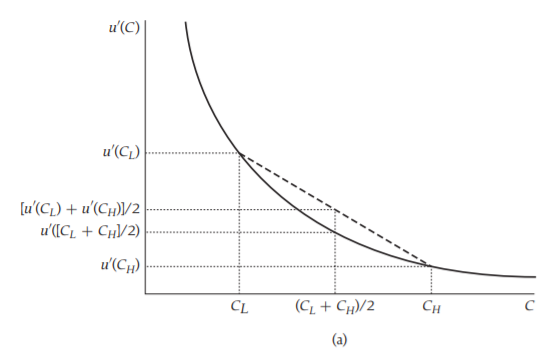
\includegraphics[width=0.8\textwidth]{subfile/attachments/4.1-risk_aversion_utility.png}
        \end{figure}
        
    \section{Random walk hypothesis}
        Assume wage is uncertain, and consumer maximizes expected utility  
        \begin{align}
            \E{U} &= \E{\sum_{t=0}^T \left(C_t - \frac{a}{2} C_t^2 \right)},
            \quad a > 0,
            \\ s.t. &\quad
            \sum_{t=0}^T \E{C_t}
            \le \E{A_0 + \sum_{t=0}^T Y_t}.
        \end{align}
        
        Form Lagrangian
        \begin{align}
            \E{\sum_{t=0}^T \left(C_t - \frac{a}{2} C_t^2 \right)} + \lambda \E{
                A_0 + \sum_{t=0}^T (Y_t-C_t),
            }
        \end{align}
        With the FOC with respect to $C_t$, we have
        \begin{align}
            \frac{\partial \L}{\partial C_t} = 0
            \implies
            \E{1 + a C_t} = \lambda
            &\implies
            \E{1 + a C_t}
            = \E{1 + a C_{t+1}}
            \\
            &\implies
            C_t
            = \Et{C_{t+1}}
            = C_{t+1} - e_{t+1},
            \quad \Et{e_{t+1}} = 0
            \\
            &\implies
            C_{t+1} = C_t + e_{t+1},
        \end{align}
        
        implying consumption follows a random walk.
        
\end{document}
